\section{Mutations of polygons and Laurent polynomials}\label{sec:combinatorics}
In this section, we give the necessary background on mutations and define maximally mutable Laurent polynomials.
	\subsection{Mutations of polygons}\label{sec:mutationsofpolygons}
Let $M$ be a two-dimensional lattice with dual lattice $N$.
	\begin{Definition}\label{def:Fanopolygon}
		A Fano polygon is a full-dimensional lattice polygon $P \subset M_\RR$ such that $0$ is in the strict interior of $P$, and the vertices of $P$ are primitive lattice points.
	\end{Definition}
For any edge $E$ of $P$, the number of lattice points on $E$ minus one is called the \emph{lattice length}~$\ell_E$ of $E$. Let $u_E \in N$ be the primitive inward normal vector corresponding to $E \subset P$, then the positive integer $-\langle u_E, E \rangle$ is called the \emph{lattice height} $h_E$ of $E$.
$P$ is \emph{reflexive} if $h_E= 1$ for all edges $E$. Define $m_E$, $r_E$ to be the unique positive integers such that
\[
\ell_E=m_Eh_E+r_E, \qquad 0 \leq r_E<h_E.
\]
We call $r_E$ the \emph{residual length} of the edge $E$. Let $\sigma_E$ be the cone over the edge $E$.
If $r_E=0$, then $\sigma_E$ is called a $T$-cone. If $r_E=0$ and $m_E=1$ (or in other words $\ell_E=h_E$), $\sigma_E$ is called a primitive $T$-cone. If $\ell_E<h_E$, $\sigma_E$ is called a $R$-cone.
In general, we may (non-uniquely) subdivide $\sigma_E$ into $m_E$ primitive $T$-cones and zero or one $R$-cones, depending on whether $r_E$ is zero or nonzero.
Fixing such a subdivision, we say that a lattice point of $P$ is \emph{residual} if it is either the origin or interior to an $R$-cone. The number of residual points of $P$ is independent of the subdivision.
	\begin{Definition}
	A $T$-polygon is a Fano polygon such that every edge $E$ of $P$ satisfies $r_E=0$. Equivalently, the lattice length $\ell_E$ is divisible by the lattice height $h_E$.
\end{Definition}
As mentioned in the introduction, the classification of orbifold del Pezzo surfaces admitting a toric degeneration is conjecturally mirror to the classification of Fano polygons up to an appropriate equivalence relation. This equivalence relation is called mutation: while it is a bit technical to define, the idea behind it is rather simple, see Figure~\ref{fig:combinatorialmutation}.
	\begin{Definition}\label{mutationdef}
		Let $P \subset M$ be a Fano polygon and let $v \in N$ be a primitive vector. Choose a~line segment $F \subset v^{\perp} \subset M$ and write $P_d$
		for the slice of $P$ at height $d$ with respect to $v$. Suppose that for all $d<0$ we can decompose $P_d=R_d+(-d)F$ as a Minkowski sum for
		some line segment $R_d$ (where we allow $R_d =\varnothing$).
		Then we say that $P$ is mutable with respect to~$(v, F)$, and define the mutation of $P$ with respect to $(v, F)$ to be
		\[
		Q=\text{conv} \biggl( \bigcup_{d<0} R_d \cup \bigcup_{d\geq 0}(P_d+dF) \biggr).
		\]
		We call $F$ the factor of the mutation, and we say that two polygons $P$, $Q$ are {\it mutation equivalent} if there is a sequence of mutations
		of polygons starting with $P$ and ending with $Q$.
	\end{Definition}
	Keeping the notation of Definition~\ref{mutationdef}, suppose $F=kF'$ for some primitive line segment $F'$ and positive integer $k$ and suppose
	that $P$ is mutable with respect to $(v, F)$. Informally, $Q$ is obtained from $P$ by contracting $k$ primitive $T$-cones on one edge of $P$ and adding $k$
	primitive $T$-cones on the opposite edge of $P$.
	In particular, the condition for $P$ to be mutable with respect to $(v, F)$ means that there is an edge of $P$ perpendicular to $v$
	long enough to allow for the contracting of $d$ copies of $F$, where $d$ is the height of $d$ with respect to $v$ (see Figure~\ref{fig:combinatorialmutation} for an example with $k=1$ and $d=3$)
	\begin{figure}[t]
		\centering
		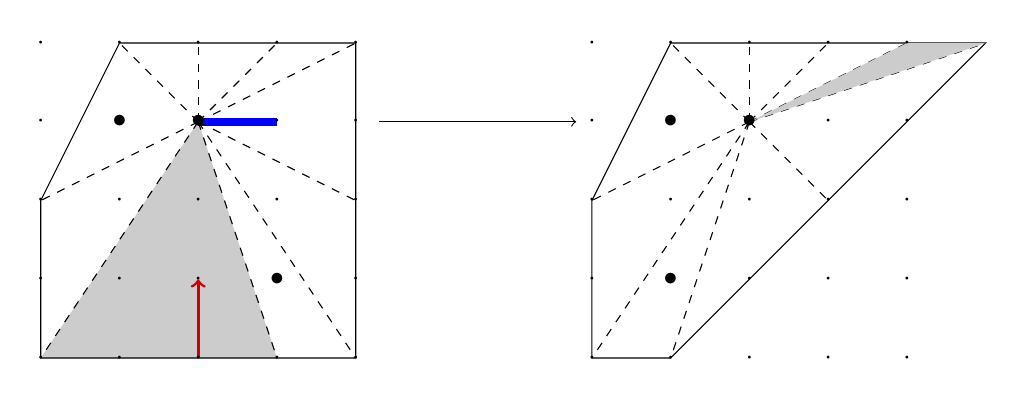
\begin{tikzpicture}[scale=1]
			\begin{scope}[blend mode=multiply]
				\draw (-2,-1) -- (-2,-3) -- (2,-3) -- (2,1)--(-1,1)--(-2,-1);
				\draw[dashed] (0,0)--(2,1);
				\draw[dashed] (0,0)--(1,-3);
				\draw[dashed] (0,0)--(0,1);
				\draw[dashed] (0,0)--(1,1);
				\draw[dashed] (0,0)--(-1,1);
				\draw[dashed] (0,0)--(-2,-1);
				\draw[dashed] (0,0)--(-2,-3);
				\draw[dashed] (0,0)--(2,-3);
				\draw[dashed] (0,0)--(2,-1);
				\draw[line width=2.7pt, blue] (0,0)--(1,0);
				\draw[->, line width=1pt, red] (0,-3)--(0,-2);
				\fill[black!20] (0,0) -- (-2,-3) -- (1,-3) -- (0,0);
				\node at (-1,-2) {$\cdot$};
				\node at (0,-2) {$\cdot$};
				\node at (1,-2) {$\bullet$};
				\node at (-2,-2) {$\cdot$};
				\node at (-1,-1) {$\cdot$};
				\node at (0,-1) {$\cdot$};
				\node at (1,-1) {$\cdot$};
				\node at (2,-1) {$\cdot$};
				\node at (-2,-1) {$\cdot$};
				\node at (-2,0) {$\cdot$};
				\node at (-2,1) {$\cdot$};
				\node at (-1,0) {$\bullet$};
				\node at (0,0) {$\bullet$};
				\node at (1,0) {$\cdot$};
				\node at (2,0) {$\cdot$};
				\node at (-1,1) {$\cdot$};
				\node at (0,1) {$\cdot$};
				\node at (1,1) {$\cdot$};
				\node at (2,1) {$\cdot$};
				\node at (2,-2) {$\cdot$};
				\node at (0,-3) {$\cdot$};
				\node at (1,-3) {$\cdot$};
				\node at (2,-3) {$\cdot$};
				\node at (-2,-3) {$\cdot$};
				\node at (-1,-3) {$\cdot$};
			\end{scope}
			\begin{scope}[xshift=7cm]
				\draw (-1,1)--(-2,-1) -- (-2,-3) -- (-1,-3) -- (3,1)--(-1,1);
				\draw[dashed] (0,0)--(2,1);
				\draw[dashed] (0,0)--(0,1);
				\draw[dashed] (0,0)--(1,1);
				\draw[dashed] (0,0)--(-1,1);
				\draw[dashed] (0,0)--(1,-1);
				\draw[dashed] (0,0)--(3,1);
				\draw[dashed] (0,0)--(-1,-3);
				\draw[dashed] (0,0)--(-2,-1);
				\draw[dashed] (0,0)--(-2,-3);
				\fill[black!20] (0,0) -- (3,1) -- (2,1) -- (0,0);
				\node at (-1,-2) {$\bullet$};
				\node at (0,-2) {$\cdot$};
				\node at (1,-2) {$\cdot$};
				\node at (-2,-2) {$\cdot$};
				\node at (-1,-1) {$\cdot$};
				\node at (0,-1) {$\cdot$};
				\node at (1,-1) {$\cdot$};
				\node at (2,-1) {$\cdot$};
				\node at (-2,-1) {$\cdot$};
				\node at (-2,0) {$\cdot$};
				\node at (-2,1) {$\cdot$};
				\node at (-1,0) {$\bullet$};
				\node at (0,0) {$\bullet$}{};
				\node at (1,0) {$\cdot$};
				\node at (2,0) {$\cdot$};
				\node at (-1,1) {$\cdot$};
				\node at (0,1) {$\cdot$};
				\node at (1,1) {$\cdot$};
				\node at (2,1) {$\cdot$};
				\node at (2,-2) {$\cdot$};
				\node at (0,-3) {$\cdot$};
				\node at (1,-3) {$\cdot$};
				\node at (2,-3) {$\cdot$};
				\node at (-2,-3) {$\cdot$};
				\node at (-1,-3) {$\cdot$};
			\end{scope}
			\draw[->] (2.3,0) -- (4.8,0);
		\end{tikzpicture}
		\caption{Mutation of the polygon $P$ with respect to mutation data $\textcolor{red}{v}=(0,1)$, $\textcolor{blue}{F}=\Newt(1+x)$. The mutation contracts a grey $T$-cone on the left and adds a grey $T$-cone on the right. Residual lattice points in bold.}
		\label{fig:combinatorialmutation}
	\end{figure}
	By \cite[Proposition 3.6]{AkhtarKasprzyk}, any mutation of a $T$-polygon again produces a $T$-polygon, so that mutation defines an equivalence relation on the set of $T$-polygons.
	\subsection{Mutations of Laurent polynomials}\label{sec:mutationsofLaurent}
	Let now $v \in N$ and $f \in \CC[v^\perp] \subset \CC[M]$. Following \cite{GrossHackingKeelClusterAlgebras} and \cite{AkhtarCoatesCorti}, we define the automorphism~\smash{$x^{m} \!\mapsto x^{m}f^{\langle {m}, {v} \rangle}$}
	of the function field $\CC(M)$. This
 induces a birational map
${\varphi_{v,f} \colon T_N \dashrightarrow T_N}$
	which we call an \emph{algebraic mutation}. We call $f$ the \emph{factor} of the mutation. We will often suppress~$v$ and $f$ from notation.
	\begin{Definition}\label{def:AlgebraicMutation}
		Given a Laurent polynomial $g \in \CC[M]$, we say that $g$ is {\it mutable} with respect to an algebraic mutation $\varphi$ if $\varphi^*(g)\in \CC[M]$, i.e., $\varphi^*(g)$ is again a Laurent polynomial, and call~$\varphi^*(g)$ a \emph{mutation} of $g$.

		Given $g, g' \in \CC[M]$, we say that $g$ and $g'$ are \emph{mutation equivalent} if there exist algebraic mutations $\varphi_i$ for $1 \leq i \leq n$ and Laurent polynomials $g_i \in \CC[M]$ for $0 \leq i \leq n$ such that~${g_0=g}$, ${g_n=g'}$ and $\varphi_i^*g_{i-1}=g_{i}$ for all $i$.
	\end{Definition}

	Let us interpret mutability more concretely. Fix mutation data $v$ and $f$ as before. Taking the inner product with $v$ gives a $\ZZ$-grading of $M$ by height, so we may write $g=\sum_{d=-h}^m g_d$ where~$g_d$ is the sum of the monomials of $g$ at height $d$.
	Extend $v$ to a basis $e_1=v$, $e_2$ for $N$ and set $x=x^{e_2^*}$ and $y=x^{e_1^*}$. The factor $f$ is then a Laurent polynomial in $x$, and $\varphi_f^*(g_d)=g_df^{d}$. It follows that $g \in \CC[M]$ is mutable with respect to $\varphi_f$ if and only if $g_{-d}$ is divisible by \smash{$f^{d}$} for~${d>0}$.
	If $f$ is a monomial, then every Laurent polynomial is mutable with respect to $\varphi_f$, and we call such mutations \emph{trivial}. If a factor is of the form $(\lambda + x^u)$ for some $\lambda \in \CC^\times$ and {primitive} $u \in M$, we call the mutation \emph{standard}. It is clear that any factor is a product of standard and trivial factors.
	It follows easily from the definitions that a mutation of Laurent polynomials induces a mutation of their Newton polygons.
	However, the converse is false, it is not true that every mutation of $\Newt(g)$ is induced by a mutation of $g$ as the following example shows:
		\begin{figure}
		\centering
		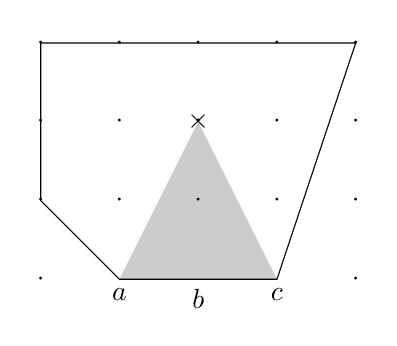
\begin{tikzpicture}[scale=1]
				\begin{scope}[blend mode=multiply]
				\draw (-2,-1) -- (-1,-2) -- (1,-2) -- (2,1)--(-2,1)--(-2,-1);
				\draw(-1,-2) node[below]{$a$};
				\draw(0,-2) node[below]{$b$};
				\draw(1,-2) node[below]{$c$};
				\node(-1,-2) {$\cdot$};
				\node(0,-2) {$\cdot$};
				\node(1,-2) {$\cdot$};
				\node at (-2,-2) {$\cdot$};
				\node at (-1,-1) {$\cdot$};
				\node at (-2,-1) {$\cdot$};
				\node at (-2,0) {$\cdot$};
				\node at (-2,1) {$\cdot$};
				\node at (0,-1) {$\cdot$};
				\node at (1,-1) {$\cdot$};
				\node at (2,-1) {$\cdot$};
				\node at (-1,0) {$\cdot$};
				\node at (0,0) {$\times$}{};
				\node at (1,0) {$\cdot$};
				\node at (2,0) {$\cdot$};
				\node at (-1,1) {$\cdot$};
				\node at (0,1) {$\cdot$};
				\node at (1,1) {$\cdot$};
				\node at (2,1) {$\cdot$};
				\node at (2,-2) {$\cdot$};
				\fill[black!20] (0,0) -- (-1,-2) -- (1,-2) -- (0,0);
			\end{scope}
		\end{tikzpicture}
	\caption{}
	\label{fig:NotInduced}
	\end{figure}
	\begin{Example}\label{ex:NotInduced}
		Consider the Fano polygon $P$ in Figure \ref{fig:NotInduced}. $P$ is mutable with respect to $v=(0,1)$ and $F=\Newt(1+x)$.
		We have that
$
		g_{-2}=y^{-2}\bigl(a+bx+cx^2\bigr)x^{-1}
$
		for some constants $a$, $b$, $c$.
		In order for the mutation $\text{mut}_{F, v}$ to be induced by an algebraic mutation of $g$, the Laurent polynomial $g$ would have to be mutable with respect to a standard factor $f=\lambda + x$. This is only possible if $f^2$ divides $g_{-2}$ which happens if and only if $b^2=4ac$.
	\end{Example}

We say that a Laurent polynomial $g$ is supported on $P$ if	$\Newt(g) \subset P$.
It is natural to make the following definition.

	\begin{Definition}\label{def:TveitenClass}
Let $P$ be a Fano polygon. A Laurent polynomial $g$ supported on $P$ is of \emph{Tveiten class} if every mutation of $P$ is induced by an algebraic mutation $\varphi$ of $g$.
	\end{Definition}
We remark that the notion of \emph{maximally mutable Laurent polynomials} is now usually reserved for a more restricted class of polynomials (see below), so we opted to name the polynomials in Definition~\ref{def:TveitenClass} in view of their detailed study in Tveiten's~\cite{Tveiten} work on period integrals.

	Let us investigate the consequences of this definition, keeping the same notation as before. Fix an edge $E$ of $P$ with inner normal $v$ and write $\ell_E=mh+r$ as before. $P$ is mutable with respect to $(v, kF)$ for all $1 \leq k \leq m$, where $F \subset v^\perp$ be a primitive line segment.
	These mutations can only be induced by an algebraic mutation of $g$
	if there exists a polynomial $f \in \CC[x]$ with~${\Newt(f)=mF}$ such that for all $0 \leq d \leq h$, $g_{-d}$ is divisible by $f^d$ in $\CC[M]$. This is quite restrictive: up to a unit in $\CC[M]$ we may write
	$f=\prod_{i=1}^{m} (\lambda_i + x)$ with $\lambda_i \neq 0$, so that we have (again up to a unit)
	\[
	g_{-d}=\prod_{i=1}^{m} (\lambda_i + x)^{d} \cdot r_{-d},
	\]
	 where $r_{-d} \in \CC[x]$.

	 We see from this that a Laurent polynomial $g$ of Tveiten class is mutable with respect to~$m$ (not necessarily distinct) standard factors $(\lambda_i + x)$ along the edge $E$, one for each primitive $T$-cone on $E$.
	Since $\text{deg}(r_{-h})=r<h$, it follows that any Laurent polynomial $g$ can be mutable with respect to a maximum of $m$ standard factors along $E$, this motivates the term \emph{maximally mutable} used for Laurent polynomials of Tveiten class in \cite{Tveiten}. However, following the now standard terminology, we reserve this notion for those Laurent polynomials where all of the factors have $\lambda_i \equiv 1$.
	
	\begin{Definition}\label{def:MMLP}
		Let $P$ be a Fano polygon. A Laurent polynomial $g$ supported on $P$ is \emph{maximally mutable} if every mutation of $P$ is induced by an algebraic mutation $\varphi$ of $g$ and, moreover, the factor $f$ of $\varphi$ can always be taken to be $f=(1+x^u)^k$ for a primitive generator $u \in \CC [v^\perp ]$ and some $k\in \ZZ_{>0}$.
	\end{Definition}

If $g$ is maximally mutable, we see that for $0 \leq d \leq h$, we must have up to a unit that
	\[
	g_{-d}=\prod_{i=1}^m (1+x)^{d} \cdot r_{-d}=(1+x)^{dm} \cdot r_{-d},
	\]
	where $r_{-d} \in \CC[x]$. In particular, if $P$ is a $T$-polygon, then $g_{-h}=c(1+x)^{mh}$ for some $c \in \CC$.
		\begin{Definition}\label{def:normalized}
		A maximally mutable Laurent polynomial is \emph{normalized} if the coefficient of $g$ at each vertex of $\Newt(g)$ is $1$, and the constant term of $g$ is $0$.
	\end{Definition}
We will need the following result, which is very similar to \cite[Proposition 3.7]{Coates2021}, except that we are also interested in non-normalized Laurent polynomials.
\begin{Theorem}\label{thm:MMLP}
	Let $P$ be a $T$-polygon. There is a unique normalized maximally mutable Laurent polynomial $g_P$ supported on $P$. Moreover, the set of maximally mutable Laurent polynomial supported on $P$ is the two parameter family generated by $g_P$ and
	the constant Laurent polynomial~$1$.
\end{Theorem}
\begin{proof}
\cite[Proposition 3.7]{Coates2021} shows that $P$ supports a unique normalized maximally mutable Laurent polynomial $g_P$.

Suppose now that $g$ is any maximally mutable Laurent polynomial supported on $P$. If the coefficient of $g$ at any vertex is nonzero, we may scale $g$ by a scalar $\lambda$ to make this coefficient $1$. The mutability condition then implies that $\tfrac{1}{\lambda}g$ has binomial edge coefficients, and \cite[Proposition~3.7]{Coates2021} applies to show that $g=\lambda g_P+\mu$ for some scalar $\mu$.
If the coefficient of $g$ at a vertex is zero, then the mutability condition implies that the coefficient of $g$ along any boundary lattice point of $P$ is zero as well. The same argument as in \cite[Proposition 3.7]{Coates2021} then shows that $P$ can only have a nonzero coefficient at the origin, showing that $g=\mu$ for some scalar $\mu$. This completes the proof.
\end{proof}

	\section{The geometry of maximally mutable Laurent polynomials}\label{sec:geometry}
In this section, we show that Laurent polynomials of Tveiten class and maximally mutable Laurent polynomials can naturally be identified with the global sections of a certain line bundle. While well known to experts, this does not seem to be in the literature.
We then construct the log Calabi--Yau pair $(Y, D)$ associated to a $T$-polygon $P$, and show that $Y$ has the structure of a rational elliptic surface with $D$ a fiber of type ${\rm I}_n$. We have chosen to state some of our results in more generality than necessary, in the hope that this will clarify the geometric viewpoint on maximally mutable Laurent polynomials. We assume the reader is familiar with the basics of toric geometry.

	Throughout, let $(Y_P, D_P)$ be the polarized toric surface associated to the normal fan $\Sigma_P$ of~$P$. The edges $E$ of $P$ correspond to the rays of $\Sigma_P$, which in turn correspond to the toric divisors~$D_E$ of $Y_{P}$. The distinguished ample divisor on $Y_P$ is defined as
$D_P=\sum_{E \subset P} h_ED_E$.
	We may resolve the singularities of ${Y}_P$ to obtain a smooth toric surface $\bar{Y}_P$, and we denote its toric boundary $\bar{D}$.
	There is a well-known isomorphism
	\begin{equation}\label{eq:sections}
		\Gamma(Y_P, \cO(D_P)) \cong \bigoplus_{m \in P \cap M} \CC x^m.
	\end{equation}
Any Laurent polynomial $g$ supported on $P$ defines a section of $\cO(D_P)$. Its vanishing locus $C$ is a compactification of the affine curve $g=0$ in the dense torus $(\CC^\times)^2 \subset Y_P$. If $\Newt(g)=P$, the curve $C$ does not contain any of the toric divisors and does not pass through any torus fixed point. In particular, it avoids all singular points of $Y_P$.
	It follows that the strict transform of~$C$ on $\bar{Y}_P$ is isomorphic to $C$.
	To analyze the geometry, we work locally: given an edge $E$ of $P$ with inner normal $v$, let $e_1=v$, $e_2$ be a basis for one of the two smooth cones $\sigma$ in the fan of~$\bar{Y}_P$ containing $\RR_{\geq 0}v$ and let $x=x^{e_2^*}$, $y=x^{e_1^*}$ be the corresponding basis of characters. Then $D_E$ has an open subset $U$ with coordinates $x$, $y$ in which $D_E$ has local equation $y=0$, and $x$ is a local coordinate on $D_E$ around the torus fixed point corresponding to the cone $\sigma$, giving an identification $D_E^{\rm int} \cong \CC^\times$. Any mutation factor $f \in \CC[v^\perp]$ can then be identified with a Laurent polynomial $f(x)$. In particular, a standard mutation factor is of the form $f(x)=\lambda+x$.
	
	\begin{Definition}\label{def:mutablecycle}
		Suppose that $g$ is a Laurent polynomial supported on $P$ which is mutable with factor $(\lambda +x)$, and let $A$ be the point on $D_E$ where $\lambda+x=0$, i.e., the point with local coordinates $(-\lambda, 0)$. Then we say that $g$ is mutable with respect to $A$.

		Similarly, if $g$ is mutable with factor $(\lambda+x)^m$ for some positive integer $m$, we say that $g$ is mutable with respect to $m A$.
		The set of all points with respect to which $g$ is mutable defines a~zero cycle $Z$ supported on the interior of the toric boundary of $Y_P$, called the mutable cycle of~$g$.
	\end{Definition}
	We see that a Laurent polynomial $g$ with $\Newt(g)=P$ is of Tveiten class if and only if the mutable cycle has exact degree $m_E$ along the edge $E$, the maximal possible. The polynomial~$g$ is maximally mutable if and only if in addition the mutable cycle $Z$ is supported on the points $-1 \in D_E^{\rm int} \cong \CC^\times$ for $E \subset P$.
We now introduce the language of Looijenga pairs, which will simplify our discussion.
Following~\cite{Friedman, GrossHackingKeelLooijengapairs}, a Looijenga pair is a smooth projective surface $Y$ together with a singular anticanonical divisor $D$ with at worst nodal singularities. The divisor~$D$ is either a~nodal curve, or a cycle of~$n$ rational curves. $Y$ is necessarily rational, so we have an isomorphism $\Pic(Y) \cong H^2(Y, \ZZ)$.
If $Y$ is a toric surface with $D=Y \setminus (\CC^\times)^2$ its toric boundary, then $(Y,D)$ is called a {\it toric pair}.
Given a Looijenga pair $(Y, D)$, there are two elementary operations to produce another Looijenga pair:
\begin{itemize}\itemsep=0pt
	\item
	Let $p \colon Y' \rightarrow Y$ be the blowup of $Y$ at a smooth point of $D$. Denoting by $D'$ the strict transform of $D$, the pair $\bigl(Y', D'\bigr)$ is again a Looijenga pair. The map $p$ is called an \emph{interior blowup}.
	\item
	Let $p \colon Y' \rightarrow Y$ the blowup of a node of $D$. Denoting by $D'$ the reduced inverse image of~$D$, the pair $\bigl(Y', D'\bigr)$ is again a Looijenga pair. The map $p$ is called a \emph{corner blowup}.
\end{itemize}
	In the literature, corner blowups are often called toric blowups. To avoid confusion, we reserve this term for the blowup of a toric surface along a torus fixed point (which is a special case of a~corner blowup).
	We say that $(Y, D)$ is positive definite (negative definite, semi-definite,~\dots) if the intersection matrix of the components of $D$ is positive definite (negative definite, semi-definite,~\dots). A matrix is strictly negative semi-definite if it is negative semi-definite but not negative definite.
We will often identify a point $A \in D^{\rm int}$ with the corresponding point $E \cap \tilde{D}$ on the strict transform $\tilde{D}$ (where $E$ is the exceptional divisor of an interior blowup). In particular, the blowup of $m A$ is understood as $m$ iterated blowups at $A$.
We now aim to give a~geometric interpretation of maximal mutability.

 Let $P$ be a Fano polygon, and let $C$ be the vanishing locus of a section of $\cO(D_P)$ on the smooth toric surface $\bigl(\bar{Y}_P, \bar{D}\bigr)$, and let $A$ be a point in the intersection $\bar{D}^{\rm int} \cap C$. Let $p \colon (Y, D) \rightarrow \bigl(\bar{Y}_P, \bar{D}\bigr)$ be the blow up $kA$, and denote the exceptional classes $E_i$, for $1 \leq i \leq k$.
\begin{Lemma}\label{lem:mutabilitygeometric}
	The curve $C$ is the vanishing locus of a section of the line bundle
$
	p^*\cO(D_P)-\sum_{i=1}^k h E_i
$
	 on $Y$ if and only if in local coordinates $x$, $y$ centered at $A$, the curve $C$ has an equation of the form
	\begin{equation}\label{eq:23}
		\sum_{i=1}^hc_i y^ix^{k(h-i)}+\text{$($terms of degree $>kh)$}=0
	\end{equation}
for some constants $c_i$ and where $\deg(x)=1$, $\deg(y)=k$.
\end{Lemma}
\begin{proof}
	We may write the defining equation of $C$ as $\sum_{i,j \geq 0} a_{i,j} x^i y^j=0$. $C$ extends to a section of~${p^*D_P-hE_i}$ if and only if $A$ is a point of multiplicity at least $h$, i.e., $a_{i,j}=0$ for $i+j<h$.
	Locally, the blowup of $A$ is given by the map $\pi_1 \colon (u,v) \mapsto (u, uv)$, and the corresponding section~$C_1$ of $p^*D_P-hE_i$ has equation
$\sum_{i,j \geq 0} a_{i,j} u^{i+j-h}v^j=0$
	 in these coordinates. The point lying over~$A$ has coordinates $(u,v)=(0,0)$, so we see that $C_1$ extends to a section of $p^*D_P-hE_1-hE_2$ if and only if $C_1$ has a point of multiplicity at least $h$ at $(0,0)$, i.e., $a_{i, j}=0$ for $i+2j<2h$.
	Continuing in a similar fashion, we see that $C$ extends to a section of~\smash{$p^*D_P-\sum_{i=1}^k h E_i$} if and only if $a_{i,j}=0$ for $i+kj<kh$.
	This happens if and only if $C$ is of the form \eqref{eq:23}.
\end{proof}

Let now $Z$ be a zero cycle, supported on $\bar{D}^{\rm int}$, and let $k_E$ be the degree of $Z$ along the edge~$\bar{D}_E$.
Define $\pi \colon \tilde{Y}_Z \rightarrow \bar{Y}_P$ to be the blowup of $Z$. The exceptional locus is a disjoint union of chains of $\PP^1$s. Each such chain is of the form $C_1+\dots +C_r$, where $C_1^2=-1$, $C_i^2=-2$ for $i>1$, and $r$ is the multiplicity of the corresponding point in $Z$. For $1 \leq i \leq r$, we define $E_i=C_1+\dots+C_i$, and call the $E_i$ the exceptional classes of the blowup. Note that $E_i^2=-1$ for all $i$. Define the line bundle
\[
L=\pi^*D_P-\sum_{E\subset P} \sum_{i=1}^{k_E} h_EE_i.
\]
	\begin{Theorem}\label{thm:MMLPassections}
There is a one-to-one correspondence between Laurent polynomials $g$ supported on $P$ whose mutable cycle contains $Z$, and global sections of $L$.
\end{Theorem}
\begin{proof}
	Let $A \in \Supp(Z) \cap D_E$. Recall that we may choose a local coordinate chart $U$ centered around a torus fixed point on $D_E$ such that $D_E$ has equation $y=0$ and $A=(-\lambda, 0)$ for some constant $\lambda$. By definition, the mutable cycle of $g$ contains $kP$ if and only if we can write
	\[
	g=	
	\sum_{i=-h_E}^{0}c_i{y^{i}}(\lambda+x)^{-ki}{r}_{i}(x)+\sum_{i=1}^m {y^{i+h_E}}{r}_i(x)
	\]
	for some constants $c_i$, and Laurent polynomials $r_i(x)$.
	Multiplying through by a monomial, we see that $g$ is mutable at $kA$ if and only if the corresponding section $C$ of $\cO(D_P)$ (under the isomorphism \eqref{eq:sections}) is locally defined by an equation of the form
	\[	
	\sum_{i=0}^{h_E}c_i{y^{i}}(\lambda+x)^{k(h_E-i)}{r}_{i}(x)+\sum_{i=1}^m {y^{i+h_E}}{r}_i(x)=0
	\]
	for some constants $c_i$ and polynomials $r_i(x)$.
	Applying the coordinate change $x \mapsto x-\lambda$, we see that $C$ is mutable at $kA$ if and only if it has a local equation of the form
	\[	
	\sum_{i=0}^{h_E}c_i{y^{i}}x^{k(h_E-i)}+\text{(terms of degree $>kh_E$)}=0.
	\]
	By Lemma~\ref{lem:mutabilitygeometric}, this happens if and only if $g$ extends to a section of $\pi^*D_P-\sum_{i=1}^k h_E E_i$. Repeating the argument for all $A \in \Supp(Z)$ shows that $g$ extends to a section of $L$ if and only if the mutable cycle of $g$ contains $Z$.
	\end{proof}

In particular, by taking $Z$ to be maximal -- in the sense that $Z$ has degree $m_E$ along $D_E$ -- we can view Laurent polynomials of Tveiten class with mutable cycle $Z$ as the space of global sections of a certain line bundle. The most important case for us if $Z$ is supported on the points~${[1:-1] \in D_E}$, which corresponds to the maximally mutable Laurent polynomials.
	\begin{Corollary}
		Let $P$ be a Fano polygon. Let $\bigl(\bar{Y}_P, \bar{D}\bigr)$ be the associated smooth toric surface. Let~\smash{$p \colon \bigl(\tilde{Y}_Z, D\bigr) \rightarrow \bigl(\bar{Y}_P, \bar{D})$} be the Looijenga pair obtained by $m_E$ blowups at the point ${[-1:1] \in D_E}$, for every edge $E \subset P$. Let $E_i$ denote the exceptional classes of the blowups. There is a~$1$-$1$ correspondence between maximally mutable Laurent polynomials $g$ supported on~$P$ and global sections of
$p^*D_P-\sum_{E \subset P}\sum_{i=1}^{m_E} h_E E_i$,
		where $E \subset P$ ranges over all edges of $P$.
	\end{Corollary}
\begin{proof}
	Immediate from Theorem~\ref{thm:MMLPassections}.
\end{proof}

We now study the pencil of sections $\Gamma_g \subset |D_P|$ generated by $g$ and the constant Laurent polynomial $1$. Note that the vanishing locus of the section corresponding to $1$ is precisely $D_P$.
\begin{Lemma}\label{lem:baseschemevsmutablecycle}
	Let $P$ be a $T$-polygon, and $g$ with $\Newt(g)=P$ a Laurent polynomial of Tveiten class. Then the base scheme of the pencil $\Gamma_g$ and the mutable cycle of $g$ are supported on the same points.
\end{Lemma}
\begin{proof}
	Let $D$ be the toric boundary of the singular toric surface $Y_P$. The zero scheme of ${1 \in \cO(D_P)}$ is the divisor $D_P$, hence the base scheme of $\Gamma_g$ is supported on the points $D \cap \{g=0\}$. As before, for a fixed edge $E$ of $P$, we have local coordinates $x$, $y$ in which $D_E$ has equation~${y=0}$ and
	\[
	g=\prod_{i=1}^{m} (\lambda_i + x)^{h} \cdot r(x) +\text{(monomials involving $y$)}
	\]
	for some polynomial $r(x)$, and since $P$ is a $T$-polygon, $r(x) \equiv 1$. It follows that the intersection~${D_E \cap \{g=0\}}$ consists of the points $(x, y)=(-\lambda_i, 0)$, which coincides with the support of the mutable cycle of $g$ on $D_E$.
\end{proof}

We note however that the mutable cycle does not coincide with the base scheme of $\Gamma_g$ as soon as $P$ has an edge at height greater than one.
\begin{Lemma}\label{lem:resolutionofsingularities}
Suppose that $P$ is a $T$-polygon, and that $g$ is a Laurent polynomial of Tveiten class with $\Newt(g)=P$. Suppose that a point $A$ appears in the mutable cycle of $g$ with multiplicity~$k$. Then
\begin{enumerate}\itemsep=0pt
	\item[$(1)$] the basepoint $A$ of $\Gamma_g$ can be resolved by a composition $p \colon \bigl(\tilde{Y}, \tilde{D}\bigr) \rightarrow \bigl(\bar{Y}_P, \bar{D}\bigr)$ of $k$ interior blowups at $A$ $($see Figure~{\rm\ref{fig:h-uplepoint}}$)$.
	\item[$(2)$] The strict transform $\tilde{D}_P$ is a member of $p_*^{-1}\Gamma_g$ and
	\[p_*^{-1}\Gamma_g \subset \left|p^*\cO(D_P)-\sum_{i=1}^{k} h_E E_i\right|.
	\]
\end{enumerate}
\end{Lemma}
\begin{proof}
$A$ lies in the interior of a toric divisor $D_E$ corresponding to an edge $E$, let $h=h_E$.
As before, we may choose local coordinates $x$, $y$ such that $D_E$ has equation $y=0$. Suppose $A$ corresponds to $\lambda \in \CC^\times \cong D_E$. By assumption, $g$ locally has an equation of the form
\[
\sum_{i=0}^h y^i(x-\lambda)^{k(h-i)}r_i(x)+O\bigl(y^{h+1}\bigr)=0.
\]
It follows that $\Gamma_g$ has a local equation
\[
s\left(\sum_{i=0}^h y^i(x-\lambda)^{k(h-i)}r_i(x)+O\bigl(y^{h+1}\bigr)\right)+ty^h=0
\]
for $[s:t]\in \PP^1$.
Locally, the blowup of $A$ is given by the map $p_1 \colon (u,v) \mapsto (u, v(u-\lambda))$. Therefore, the strict transform of the pencil is given by
 \[
s\left(\sum_{i=0}^h v^i(u-\lambda)^{(k-1)(h-i)}r_i(u)+O\bigl(v^{h+1}\bigr)\right)+tv^h=0.
 \]
We note that the only basepoint of $p_{1*}^{-1}\Gamma_g$ on the exceptional divisor $u=\lambda$ is the point ${(u,v)=(\lambda, 0)}$, the intersection of the exceptional divisor with the strict transform of $D_E$.
After~$k$ blowups at $(\lambda, 0)$, the strict transform $p_*^{-1}\Gamma_g$ is given by
 \[
 s\left(\sum_{i=0}^h v^ir_i(u)+O\bigl(v^{h+1}\bigr)\right)+tv^h=0.
 \]
 $P$ is a $T$-polygon and $g$ is of Tveiten class, therefore $r_0(u)$ is a product of factors of the form~${(u-\lambda_i)^h}$, with $\lambda_i \neq \lambda$. It follows that $r_0(\lambda) \neq 0$, and so $p_*^{-1}\Gamma_g$ has no basepoint on the exceptional divisor $u=\lambda$, which proves the first claim.
The strict transform of $D_P$ under~$p$ has equation $v^h=0$, which is the member of $p_{*}^{-1}\Gamma_g$ corresponding to $[s:t]=[0:1]$. Finally, the proof shows that each blowup removes a basepoint of multiplicity $h=h_E$ from $\Gamma_g$, so that%
	\[
	p_*^{-1}\Gamma_g \subset \left|p^*D_P-\sum_{i=1}^{k} h_E E_i\right|.\tag*{\qed}
\] \renewcommand{\qed}{}
\end{proof}

\tikzset{every picture/.style={line width=0.75pt}} %set default line width to 0.75pt
\begin{figure}[t]\centering
	\begin{tikzpicture}
		
		\draw [blue] (-2,0) -- (2,0);
		\draw (-2,-1.5) .. controls (-1,0.5) and (1,0.5).. (2,-1.5);
		\draw (-1.5,-1.5) .. controls (-1,0.5) and (1,0.5).. (1.5,-1.5);
		\draw (-2,1.5) .. controls (-1,-0.5) and (1,-0.5) .. (2,1.5);
		\filldraw [red] (0,0) circle (2pt);
		\draw [blue] (3.5,0) -- (7.5,0);
		\draw [green] (5.5,-1.5) -- (5.5,1.5);
		\draw (4.5, -1) -- (6.5, 1);
		\draw (5, -1) -- (6, 1);
		\draw (4.5, 1) -- (6.5, -1);
		\filldraw [red] (5.5,0) circle (2pt);
		\draw [blue] (9,0) -- (13,0);
		\draw [green] (11,-1.5) -- (11,1.5);
		\draw (10, -0.5) -- (12, -0.5);
		\draw (10, -1) -- (12, -1);
		\draw [green] (10, 1) -- (13, 1);
		\draw (10, 0.5) -- (12, 0.5);
		\filldraw [red] (11,0) circle (2pt);
		\draw [->] (3.25,0) --(2.25,0);
		\draw [->] (8.75,0) --(7.75,0);
	\end{tikzpicture}
		\caption{A triple point with two-fold tangency (along the blue divisor) and its resolution, exceptional divisors in green.}
\label{fig:h-uplepoint}
\end{figure}

We deduce the following theorem.
\begin{Theorem}
	Let $P$ be a $T$-polygon, and let $g$ a maximally mutable Laurent polynomial with~${\Newt(g)=P}$. Let $p \colon \tilde{Y}_Z \rightarrow \bar{Y}_P$ be the blowup of the mutable cycle $Z$ of $g$.
	\begin{enumerate}[$(a)$]\itemsep=0pt
	\item $p$ is a composition of interior blowups, and in particular $\bigl(\tilde{Y}_Z, \tilde{D}\bigr)$ is a Looijenga pair.
	\item The linear system $p_*^{-1}\Gamma_g$ defines a morphism $\pi \colon \tilde{Y}_Z \rightarrow \PP^1$ which is an elliptic fibration with connected fibers, and $\pi^*(\infty)=\tilde{D}_P$.
	\end{enumerate}
\end{Theorem}
\begin{proof}
	(a) is clear from the definition of $\tilde{Y}_Z$.

	For (b), applying Lemma~\ref{lem:resolutionofsingularities} repeatedly shows that
	\begin{equation}\label{eq:stricttransformofpencil}
	p_*^{-1}\Gamma_g \subset 	\left|p^*D_P-\sum_{E \subset P}\sum_{i=1}^{m_E} h_E E_i\right|.
	\end{equation}
	Lemma~\ref{lem:baseschemevsmutablecycle} shows that the only basepoints of $\Gamma_g$ occur at the support of the mutable cycle, and Lemma~\ref{lem:resolutionofsingularities} shows that blowing up the mutable cycle removes these basepoints, so that $p_*^{-1}\Gamma_g$ is base-point-free, and defines a morphism $\pi \colon \tilde{Y}_Z \rightarrow \PP^1$. By Bertini's theorem, the general member of $p_*^{-1}\Gamma_g$ is smooth, so the general fiber of $\pi$ is smooth. By Theorem~\ref{thm:MMLPassections}, sections of $L$ correspond to maximally mutable Laurent polynomials supported on $P$, and by Theorem~\ref{thm:MMLP}, the space of maximally mutable Laurent polynomials is two-dimensional. It follows that the inclusion \eqref{eq:stricttransformofpencil} is an equality, and $p_*^{-1}\Gamma_g$ is a complete linear system. Therefore, the morphism~$\pi$ is equal to its Stein factorization, so that $\pi$ has connected fibers. The fact that the general fiber has genus~$1$ follows from Riemann--Roch, see \cite[Theorem 3.5]{Tveiten}. Finally, Lemma~\ref{lem:resolutionofsingularities} shows that~$\tilde{D}_P$ is a~member of $p_*^{-1}\Gamma_g$, so that $\pi^*(\infty)=\tilde{D}_P$ after choosing suitable coordinates on~$\PP^1$.
\end{proof}
